\section{Competition adaptation and complete prediction traces}
\label{app:competition-details}
This appendix details input construction and timing for the 434-query competition population. Linear and symmetric-log views show the full signed prediction traces.

\subsection{Frozen models and causal input construction}

We use the public Hugging Face full, event-only, and visual-only checkpoints with their released configurations and source revision. Strict state-dictionary loading and float32 inference keep each model fixed. The release identifies the checkpoint bytes but does not document complete training membership, so the evaluation represents frozen-checkpoint adaptation rather than a claim of clean zero-shot transfer.

Garl-TTC predicts the ratio of object heights at two endpoints and converts it to TTC as
\begin{equation}
 \widehat T
 =\frac{\Delta t_{\mathrm{measured}}}
 {1-\widehat h_0/\widehat h_1}.
 \label{eq:garl-height-ratio-evttc}
\end{equation}
The released configuration sets the native model field $\mathrm{dT}=0.1$\,s. For Equation~\ref{eq:garl-height-ratio-evttc}, the adapter substitutes the measured separation of each endpoint pair while leaving the released representation unchanged. The checkpoint metadata do not establish the cadence used during training.

The full and visual routes select the latest real RGB frame at or before a query, then the preceding frame closest to 100\,ms earlier. Full Garl builds one causal event window per RGB endpoint with support capped at $\min(\Delta t_{\mathrm{measured}},100\,\mathrm{ms})$. Event-only Garl uses two consecutive 100\,ms windows after startup and splits the observed causal prefix into two intervals for earlier queries. Each endpoint uses the released 20-plane, polarity-agnostic time volume. Queries without sufficient history remain gaps.

PHASE-TTC uses its declared 650\,ms causal history. The shared query population therefore compares the frozen systems under their respective temporal support.

Supplied boxes use zero-based, half-open event-plane coordinates. The adapter selects the latest box available at each endpoint; if the endpoint precedes all query-causal boxes, it uses the earliest such box and records availability at query time. Road sequences pair right Blackfly RGB with right Prophesee events. Slider uses its supplied streams and a rotation derived from camera poses because its calibration lacks a named event-to-RGB extrinsic. Calibrated intrinsics, distortion, and rotation-only ray projection map the event box into RGB; unavailable object depth precludes translational correction. A common square edge spans the endpoint boxes, with endpoint-specific event centers and the current center applied to both RGB frames.


\subsection{Published three-sequence comparison}
Table~VI of the eAP paper reports Garl-TTC on three EvTTC sequences, with an unweighted mean RTE of 10.60\% \citep{eap}. That study uses a separate labeled population; shared scenario names do not establish shared recordings or query identities. \evidence{T02}
\begin{table}[H]
\centering\small
\caption{Garl-TTC's published zero-shot relative TTC error on three EvTTC sequences, as reported in the eAP paper, Table VI. \evidence{T02}}
\label{tab:evttc-published-rte}
\begin{tabular}{@{}lr@{}}
\toprule
\textbf{Published sequence} & \textbf{RTE (\%)} \\
\midrule
CCRs2-medium & 8.31 \\
CCRs2-high & 10.56 \\
CCRm-medium & 12.93 \\
\textbf{Unweighted average} & \textbf{10.60} \\
\bottomrule
\end{tabular}
\end{table}

\begin{table}[H]
\centering\scriptsize
\caption{Garl--PHASE prediction comparisons for all ten sequences. Each entry gives shared-finite coverage and median absolute prediction difference in seconds. \evidence{T01}}
\label{tab:evttc-sequence-disagreement}
\setlength{\tabcolsep}{3.2pt}
\begin{tabular}{@{}lrrr@{}}
\toprule
\textbf{Sequence} & \textbf{Full $n/N$; med.} & \textbf{Event $n/N$; med.} & \textbf{Visual $n/N$; med.} \\
\midrule
CCRs1-low & 49/50; 0.465 & 50/50; 0.776 & 49/50; 0.213 \\
CCRs1-medium & 42/43; 0.308 & 43/43; 0.863 & 42/43; 0.200 \\
CCRs1-high & 29/30; 0.207 & 30/30; 0.519 & 29/30; 0.111 \\
CCRs2-low & 45/46; 0.221 & 46/46; 0.339 & 45/46; 0.243 \\
CCRs2-medium & 54/55; 0.178 & 55/55; 1.045 & 54/55; 0.254 \\
CCRs2-high & 58/59; 0.188 & 59/59; 0.682 & 58/59; 0.223 \\
CCRm-low & 41/42; 0.270 & 42/42; 0.703 & 41/42; 0.283 \\
CCRm-medium & 39/40; 0.151 & 40/40; 0.839 & 39/40; 0.350 \\
Slider-750 & 49/51; 0.408 & 51/51; 0.470 & 51/51; 0.258 \\
Slider-1000 & 18/18; 0.288 & 18/18; 0.119 & 18/18; 0.067 \\
\bottomrule
\end{tabular}
\end{table}


\subsection{Runtime boundary and interpretation}

\begin{table}[H]
\centering\small
\caption{Offline processing time in seconds per query. Model time covers the synchronized forward pass and host output; full time includes tensor preparation. The Garl variants ran in full/event/visual order; PHASE-TTC used its own adapter and history length. \evidence{T01}}
\label{tab:evttc-runtime}
\begin{tabular}{@{}lrrrr@{}}
\toprule
\textbf{Model} & \textbf{Model med.} & \textbf{Model P95} & \textbf{Full med.} & \textbf{Full P95} \\
\midrule
PHASE-TTC & 0.753 & 7.820 & 2.687 & 9.073 \\
Garl full & 0.039 & 0.045 & 0.542 & 1.009 \\
Garl event-only & 0.007 & 0.011 & 0.350 & 0.806 \\
Garl visual-only & 0.007 & 0.011 & 0.158 & 0.221 \\
\bottomrule
\end{tabular}
\end{table}


Timing separates tensor preparation from the synchronized model-to-host call and excludes loading, indexing, calibration, source hashing, and result serialization. The variants run once in full, event-only, visual-only order, so operating-system and HDF5 caches and GPU warm state can carry between runs. Table~\ref{tab:evttc-runtime} reports these observations alongside PHASE-TTC, whose adapter and temporal support differ.

Independent verification accounts for each planned record and replays the float32 height-to-TTC conversion. Full and visual Garl remain partial because of input gaps; event-only contains all 434 rows. Across the ten sequences, the four routes exhibit distinct signed behavior and disagreement tails. \evidence{T01}

\clearpage
\subsection{All ten sequences, with missing inputs preserved}
\begin{figure}[H]
\centering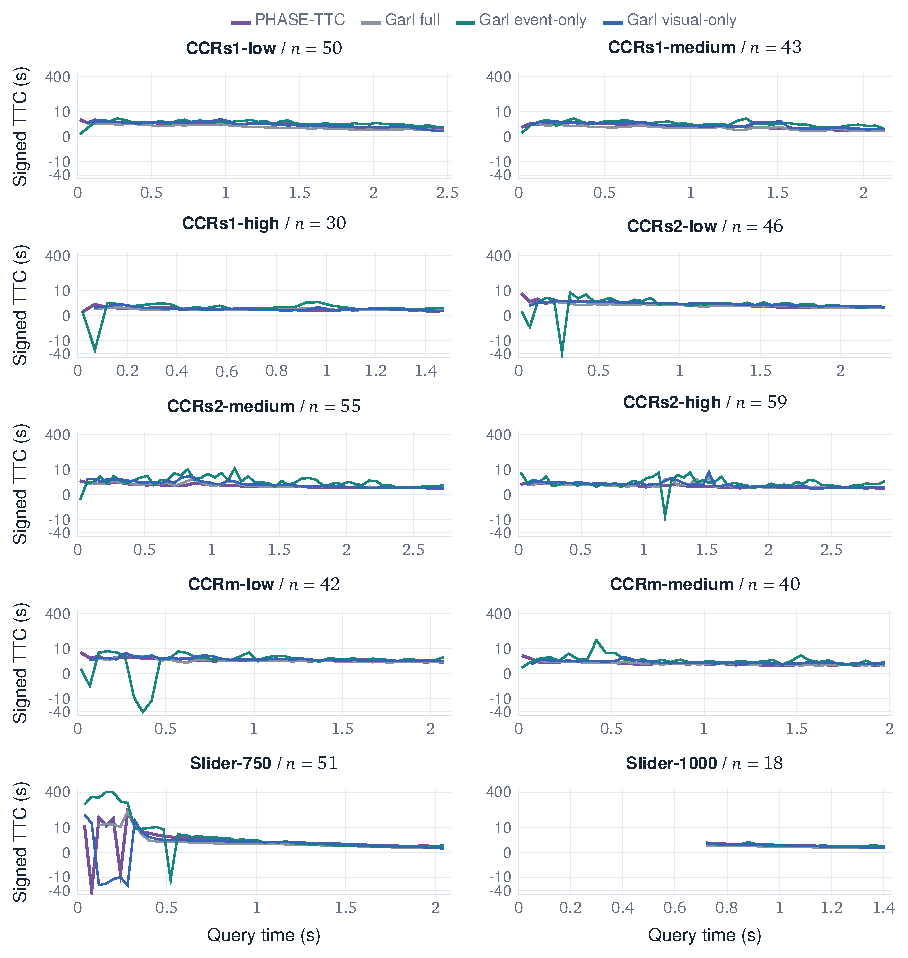
\includegraphics[width=\linewidth,height=.72\textheight,keepaspectratio]{figures/rev_competition_symlog.pdf}
\caption{\textbf{Signed predictions on a symmetric-log scale.} PHASE-TTC is purple, Garl full gray, event-only teal, and visual-only blue. All panels are linear inside $[-2,2]$\,s and logarithmic outside; gaps mark unavailable inputs. \evidence{T01}}
\label{fig:evttc-predictions-symlog}
\end{figure}
\clearpage
\begin{figure}[H]
\centering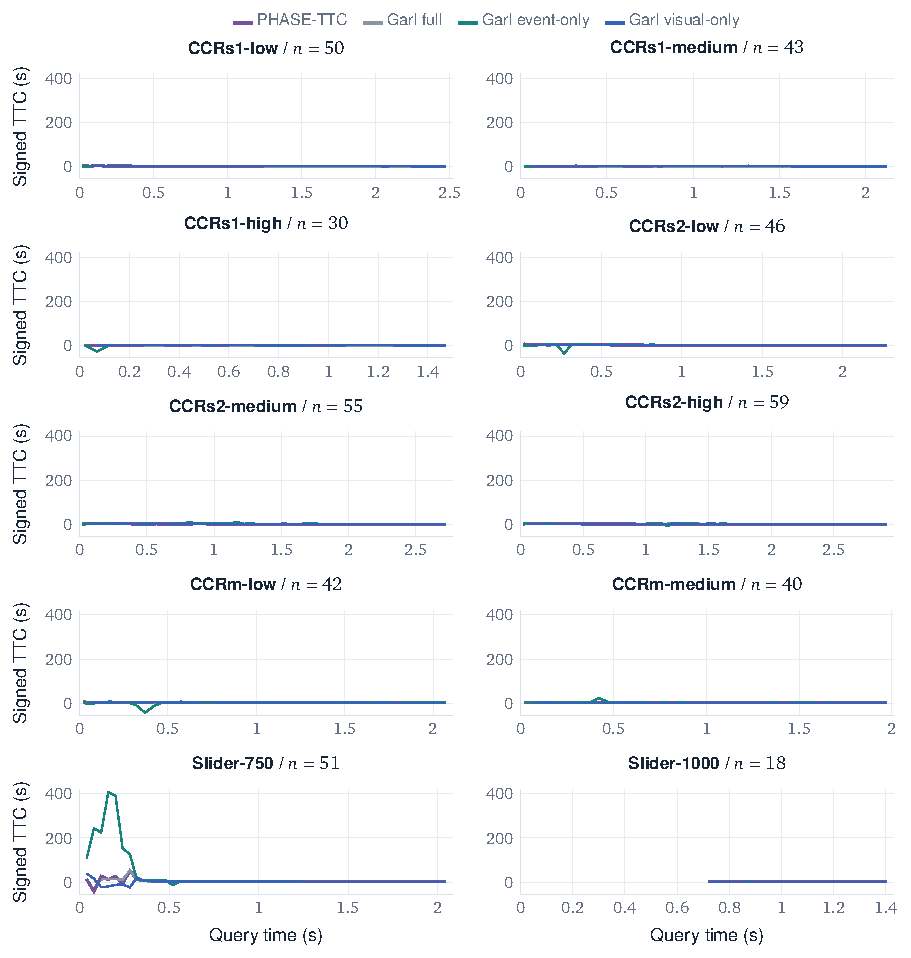
\includegraphics[width=\linewidth,height=.72\textheight,keepaspectratio]{figures/rev_competition_linear.pdf}
\caption{\textbf{Signed predictions on a common linear scale.} The same outputs as Figure~\ref{fig:evttc-predictions-symlog} show the full excursion range, which compresses the central values. \evidence{T01}}
\label{fig:evttc-predictions-linear}
\end{figure}
\FloatBarrier

\clearpage
